\documentclass[tikz,border=10pt]{standalone}
\usepackage{tikz}
\usepackage{fontspec}
\usepackage{amsmath}
\usetikzlibrary{arrows.meta, positioning, calc, decorations.pathreplacing, shapes.misc}

\begin{document}
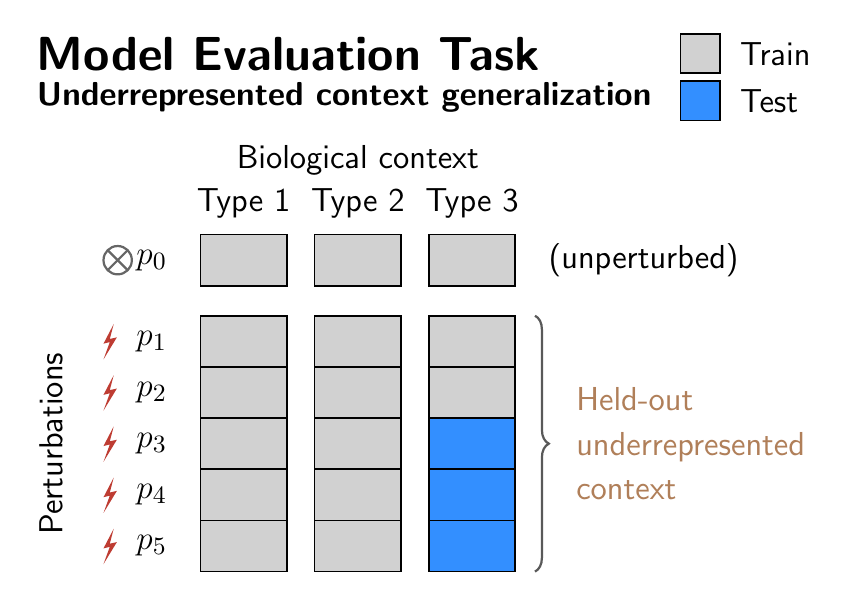
\begin{tikzpicture}[
    font=\sffamily\fontsize{13}{16}\selectfont,
    trainfill/.style={fill=black!18, draw=black, line width=0.6pt},
    testfill/.style={fill=blue!55!cyan!80, draw=black, line width=0.6pt},
    unobsfill/.style={fill=white, draw=black, line width=0.6pt},
    legendbox/.style={minimum width=5mm, minimum height=5mm, inner sep=0pt},
]

% ===== Colors =====
\definecolor{titlebrown}{RGB}{176,127,89}
\definecolor{perturbbrown}{RGB}{200,150,100}
\definecolor{contextorange}{RGB}{225,170,70}
\definecolor{testblue}{RGB}{60,120,180}
\definecolor{bolt}{RGB}{190,60,50}

% ===== Bar layout =====
% 3 columns (cell types) x 6 rows (p_0 + p_1..p_5)
% Each cell is 1.0cm wide x 0.65cm tall
\def\cellw{1.1}
\def\cellh{0.65}
\def\gap{0.35}

% x positions of column centers
\def\xA{0}
\def\xB{1.45}
\def\xC{2.90}

% y positions of row centers — row 0 at top (p_0), rows 1-5 below
% top of p_0 at y=0 (reference), cells extend downward
% For drawing, let's set p_0 top at y=0
\def\brk{0.38}  % vertical break between p_0 and p_1..p_5
\def\yP#1{-0.5*\cellh - #1*\cellh}  % center y of row #1 (0-indexed)
\def\yQ#1{-0.5*\cellh - #1*\cellh - \brk}  % center y for perturbation rows (with break)

% ===== Draw cells =====
% Row 0: p_0 (control / unperturbed) — gray across all columns
\foreach \x in {\xA, \xB, \xC} {
    \draw[trainfill] (\x - 0.5*\cellw, {\yP{0} - 0.5*\cellh}) rectangle
                     (\x + 0.5*\cellw, {\yP{0} + 0.5*\cellh});
}

% Rows 1-5 for training columns A and B — all gray (train)
\foreach \r in {1,2,3,4,5} {
    \foreach \x in {\xA, \xB} {
        \draw[trainfill] (\x - 0.5*\cellw, {\yQ{\r} - 0.5*\cellh}) rectangle
                         (\x + 0.5*\cellw, {\yQ{\r} + 0.5*\cellh});
    }
}

% Column C (held-out underrepresented): 2 train + 3 test (50% held out as test)
% p_1, p_2 train (gray); p_3, p_4, p_5 test (blue)
\foreach \r/\sty in {1/trainfill, 2/trainfill, 3/testfill, 4/testfill, 5/testfill} {
    \draw[\sty] (\xC - 0.5*\cellw, {\yQ{\r} - 0.5*\cellh}) rectangle
                (\xC + 0.5*\cellw, {\yQ{\r} + 0.5*\cellh});
}

% ===== Row labels with lightning bolts =====
% p_0: small circle with X (unperturbed)
\draw[thick, black!60] ({\xA - 0.5*\cellw - 1.05}, {\yP{0}}) circle (0.18);
\draw[thick, black!60] ({\xA - 0.5*\cellw - 1.05 - 0.13}, {\yP{0} - 0.13}) -- ({\xA - 0.5*\cellw - 1.05 + 0.13}, {\yP{0} + 0.13});
\draw[thick, black!60] ({\xA - 0.5*\cellw - 1.05 - 0.13}, {\yP{0} + 0.13}) -- ({\xA - 0.5*\cellw - 1.05 + 0.13}, {\yP{0} - 0.13});
\node[anchor=east, font=\sffamily\itshape\fontsize{13}{16}\selectfont] at ({\xA - 0.5*\cellw - 0.3}, {\yP{0}}) {$p_{0}$};

% p_1..p_5 with lightning bolt icons
\foreach \r in {1,2,3,4,5} {
    \fill[bolt] ({\xA - 0.5*\cellw - 1.15}, {\yQ{\r}}) ++(0.05,0.22) -- ++(-0.13,-0.25) -- ++(0.08,0.02) -- ++(-0.08,-0.22) -- ++(0.17,0.28) -- ++(-0.09,-0.02) -- cycle;
    \node[anchor=east, font=\sffamily\itshape\fontsize{13}{16}\selectfont] at ({\xA - 0.5*\cellw - 0.3}, {\yQ{\r}}) {$p_{\r}$};
}

% "Perturbations" rotated label on far left
\node[rotate=90, anchor=center, font=\sffamily\fontsize{13}{16}\selectfont]
    at ({\xA - 0.5*\cellw - 1.9}, {\yQ{3}}) {Perturbations};

% "(unperturbed)" next to p_0 row on the right
\node[anchor=west, font=\sffamily\fontsize{13}{16}\selectfont]
    at ({\xC + 0.5*\cellw + 0.3}, {\yP{0}}) {(unperturbed)};

% ===== Column labels =====
\node[font=\sffamily\fontsize{13}{16}\selectfont] at (\xA, 0.4) {Type 1};
\node[font=\sffamily\fontsize{13}{16}\selectfont] at (\xB, 0.4) {Type 2};
\node[font=\sffamily\fontsize{13}{16}\selectfont] at (\xC, 0.4) {Type 3};

% "Biological context" header
\node[font=\sffamily\fontsize{13}{16}\selectfont] at (\xB, 0.95) {Biological context};

% ===== Underrepresented annotation (right-side bracket/arrow to column C) =====
\draw[decorate, decoration={brace, amplitude=5pt}, thick, black!65]
    ({\xC + 0.5*\cellw + 0.25}, {\yQ{1} + 0.5*\cellh})
    -- ({\xC + 0.5*\cellw + 0.25}, {\yQ{5} - 0.5*\cellh});
\node[anchor=west, align=left, font=\sffamily\fontsize{13}{16}\selectfont, color=titlebrown]
    at ({\xC + 0.5*\cellw + 0.65}, {\yQ{3}}) {Held-out\\underrepresented\\context};

% ===== Titles (left) + Legend (right, stacked vertically) =====
\node[font=\sffamily\bfseries\fontsize{16}{19}\selectfont, color=black, anchor=west]
    at (-2.75, 2.3) {Model Evaluation Task};
\node[font=\sffamily\bfseries\fontsize{12}{15}\selectfont, color=black, anchor=west]
    at (-2.75, 1.75) {Underrepresented context generalization};

% Legend stacked vertically to the right of the title
\coordinate (legtop) at (5.8, 2.3);
\node[legendbox, trainfill] (lg1) at (legtop) {};
\node[anchor=west, font=\sffamily\fontsize{13}{16}\selectfont] at ($(lg1.east) + (0.12,0)$) {Train};

\node[legendbox, testfill] (lg2) at ($(legtop) + (0, -0.6)$) {};
\node[anchor=west, font=\sffamily\fontsize{13}{16}\selectfont] at ($(lg2.east) + (0.12,0)$) {Test};

\end{tikzpicture}
\end{document}
